\section{Level description}

The city is loosely based on Venice.

\begin{center}
  \begin{figure}[H]
    \centering
    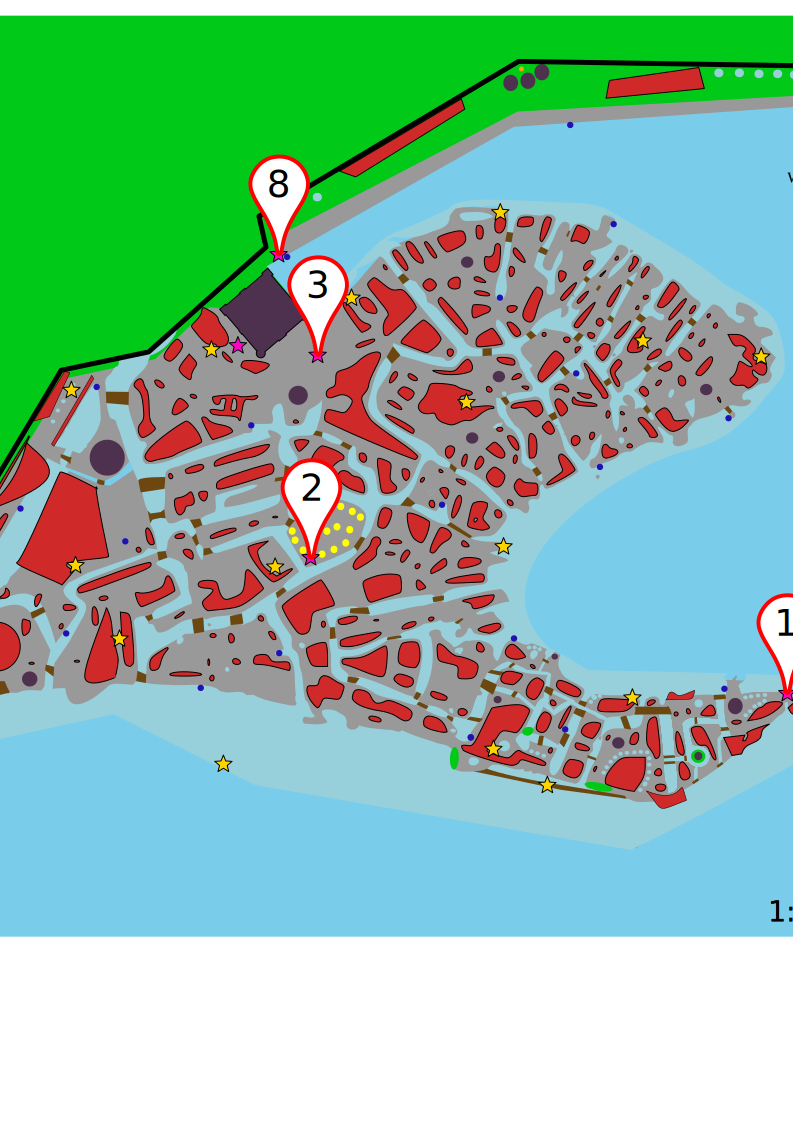
\includegraphics[width=\textwidth]{Images/Maps/dynamia}
    \caption{Map of Dynamia}
  \end{figure}
\end{center}

\newpage

\subsection{Dead end}
\begin{figure}[H]
    \centering
    \includegraphics[width=8cm]{Images/Maps/deadEnd}
  \end{figure}
Dynamia ends here, in a neighbourhood of colored houses that overlook on the canal. Some house have a view-sea and others are placed so
close themselves that there is just street that pass through them all. \\
The street isn't too wide e the house conncted to the castle is placed in front of where the street ends. 
It is short and connects the neighbourhood to a big street directed the central neighbourhoods of Dynamia. \\
At the beginng of it there is a manifests and a panel with the map of the city. 
The street is bordered by flowerbeds and fountains of all shapes but is loosely based on the \textit{Champs Elysees}.
Some small streets and dead ends are connected in its left while in its right there is canals water.
Everywhere inside it you can see a big arc of triumph at the end of the street. There beginning the real Dynamia
\begin{figure}[H]
    \centering
    \includegraphics[width=8cm]{Images/Landmarks/arcOfTriumph}
    \caption{A references images of the arc of triumph}
    For more reference images: \href{http://wastelandsteam.altervista.org/dynamia-dead-end}{http://wastelandsteam.altervista.org/dynamia-dead-end}\\Password: \textit{gld18}
  \end{figure}

\subsection{Market of Dynamia}
The Market is situated in wide square positioned in the middle of the city. It is located near many canals and it is the nerve centre of Dynamia where, everyday, people and merchants from every part of the region come to buy and sell any kind of merch. 

\subsection{Castle of Dynamia}
The castle of Dynamia is loosely based on the Sforza Castle of Milan.

\begin{figure}[H]
  \centering
  \includegraphics[width=\textwidth]{Images/Maps/castleOfDynamia}
  \caption{Map of the Castle of Dynamia}
\end{figure}

It is placed upon a rocky promontory and it is the main entrance to Dynamia from the continent. It has been designed by the court magician of Dynamia centuries ago, and it has many secret passages. The player can access some of this secret passages by solving puzzles.

It is made of stones, it has a big courtyard and two buildings: one on the west, heavily fortified, and one, more refined, on the north for the royal family. Mizar lives in the northern building, but the player can visit only the courtyard and the western area.

There are human guards and demons that patrol the castle. They are ordered to arrest any intruder. The most powerful enemy is the captain of the guards.

\subsubsection{Puzzles}
While exploring the castle, the player can choose to solve some puzzles and, by so, avoid fighting some enemies.

\subsubsection*{1. Build a machine}

In order to enter in the courtyard the player can use some debris to build a machine for Calcifer that allows him to climb the wall without being detected.

The player has different parts and he/she has to understand how to combine them.

\subsubsection*{2. Rotate the torch}

\begin{figure}[H]
  \centering
  \includegraphics[width=\textwidth]{Images/Puzzles/castleOfDynamia_2}
  \caption{Puzzle 2 in the Castle of Dynamia}
\end{figure}

The torch is a puzzle itself. The player has to rotate the torch and its parts according to the given scheme. When the player rotate a block, the upper blocks rotate too according to the scheme in figure X.Y.

\subsubsection*{3. Press the bricks}

\begin{figure}[H]
  \centering
  \includegraphics[width=\textwidth]{Images/Puzzles/castleOfDynamia_3}
  \caption{Puzzle 3 in the Castle of Dynamia}
\end{figure}

Near the torch there is a small plate with some horizontal lines. The player has to press the bricks in the corresponding position under the torch.

\subsubsection*{4. Connect the cables}

\begin{figure}[H]
  \centering
  \includegraphics[width=\textwidth]{Images/Puzzles/castleOfDynamia_4}
  \caption{Puzzle 4 in the Castle of Dynamia}
\end{figure}

There are some cables that hang under the torch. The player has to connect them in the correct pairs, according to the pattern on the plugs.

\subsection{Docking point}
\begin{figure}[H]
    \centering
    \includegraphics[width=8cm]{Images/Maps/dockingPoint}
  \end{figure}
A strict piece of terrain connect the area with the one of the castle. 
The area is fanced whit wooden poles decored with flowers except for the stairs with golden railing through you can go down to the canal.
There are small boats and gondolas attracked at this point. The water is limpid and the sun is mirrored inside it. 
In front of the bridge there is a street for the castle. 
In the center of the area there is a small street and a fountain rapresenting mizar. She keeps her right arm up holding her scepter that is a fountain. Flowers surrounded it. Behind the docking point you can see the city walls.
\begin{figure}[H]
    \centering
    \includegraphics[width=8cm]{Images/Landmarks/dockingPoint}
    \caption{A references images of a docking point}
    For more reference images: \href{http://wastelandsteam.altervista.org/dynamia-docking-point}{http://wastelandsteam.altervista.org/dynamia-docking-point}\\Password: \textit{gld18}
  \end{figure}
